\documentclass[tikz,border=10pt]{standalone}
\usepackage{tikz}

\begin{document}
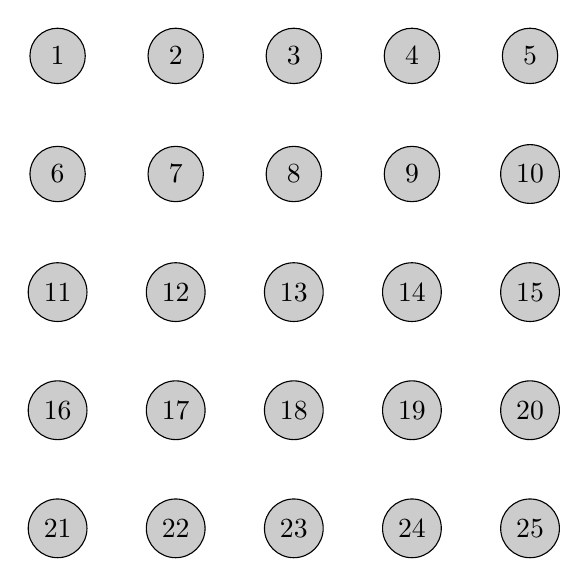
\begin{tikzpicture} [darkstyle/.style={circle,draw,fill=gray!40,minimum size=20}]
  \foreach \x in {0,...,4}
    \foreach \y in {0,...,4}
       {\pgfmathtruncatemacro{\label}{\x - 5 *  \y +21}
       %\node (\x\y) at (1.5*\x,1.5*\y) {\label};}
       \node [darkstyle]  (\x\y) at (1.5*\x,1.5*\y) {\label};}

  %\foreach \x in {0,...,4}
  %  \foreach \y [count=\yi] in {0,...,3}
  %    \draw [dashed] (\x\y)--(\x\yi) (\y\x)--(\yi\x) ;

\end{tikzpicture}
\end{document}
